\documentclass[11pt]{article}
\usepackage[margin=1in]{geometry}
\usepackage{amsmath,amssymb,booktabs,array,graphicx,float,microtype}
\usepackage[authoryear]{natbib}
\usepackage[font=small,labelfont=bf]{caption}
\usepackage{xcolor}
\usepackage{hyperref}
\emergencystretch=2em
\hypersetup{colorlinks=true,linkcolor=blue!50!black,
  citecolor=blue!50!black,urlcolor=blue!60!black}
\graphicspath{{output/}}
\newcommand{\DemandSD}{0.464}
\newcommand{\SupplySD}{0.670}
\newcommand{\MonetaryFollowerSlope}{0.0128}
\newcommand{\FiscalFollowerSlope}{0.0040}
\newcommand{\MonCostMIndex}{0.006}
\newcommand{\FisCostFIndex}{0.185}
\newcommand{\BothMIndex}{0.193}
\newcommand{\BothFIndex}{0.193}
\newcommand{\DemandMonActionIndex}{0.294}
\newcommand{\DemandFisActionIndex}{0.187}
\newcommand{\SupplyMonActionIndex}{0.271}
\newcommand{\SupplyFisActionIndex}{0.051}
\newcommand{\DemandLeaderSeparation}{0.0010}
\newcommand{\SupplyLeaderSeparation}{0.0009}
\newcommand{\BaselineGamma}{5.15e-05}
\newcommand{\BaselinePersistenceM}{0.332}
\newcommand{\BaselinePersistenceF}{0.281}
\newcommand{\GammaTenPenaltyScale}{0.011}
\newcommand{\GammaTenTransmissionScale}{9.76}
\newcommand{\BaselineMonetaryWedgeShare}{0.002}
\newcommand{\BaselineFiscalWedgeShare}{0.025}
\newcommand{\DemandFlexibleLoss}{0.2022}
\newcommand{\DemandFlexibleM}{-0.1156}
\newcommand{\DemandFlexibleF}{0.2290}
\newcommand{\DemandMonetaryLoss}{0.2029}
\newcommand{\DemandMonetaryM}{-0.0777}
\newcommand{\DemandMonetaryF}{0.2289}
\newcommand{\DemandFiscalLoss}{0.2017}
\newcommand{\DemandFiscalM}{-0.1155}
\newcommand{\DemandFiscalF}{0.1566}
\newcommand{\DemandBothLoss}{0.2023}
\newcommand{\DemandBothM}{-0.0776}
\newcommand{\DemandBothF}{0.1565}
\newcommand{\DemandCoordLoss}{0.2007}
\newcommand{\DemandCoordM}{-0.1762}
\newcommand{\DemandCoordF}{0.1574}
\newcommand{\SupplyFlexibleLoss}{0.7071}
\newcommand{\SupplyFlexibleM}{0.1722}
\newcommand{\SupplyFlexibleF}{0.0711}
\newcommand{\SupplyMonetaryLoss}{0.7071}
\newcommand{\SupplyMonetaryM}{0.1139}
\newcommand{\SupplyMonetaryF}{0.0709}
\newcommand{\SupplyFiscalLoss}{0.7070}
\newcommand{\SupplyFiscalM}{0.1724}
\newcommand{\SupplyFiscalF}{0.0584}
\newcommand{\SupplyBothLoss}{0.7070}
\newcommand{\SupplyBothM}{0.1140}
\newcommand{\SupplyBothF}{0.0584}
\newcommand{\SupplyCoordLoss}{0.7066}
\newcommand{\SupplyCoordM}{0.1469}
\newcommand{\SupplyCoordF}{0.0251}
\newcommand{\BilateralRadius}{0.9411}
\newcommand{\SearchStarts}{6}
\newcommand{\SearchMaxDistance}{4.99e-11}

\newcommand{\NKBackwardMatch}{0.00e+00}
\newcommand{\NKDistinctSolutions}{1}
\newcommand{\NKSearchAttempts}{7}
\newcommand{\NKFlexibleM}{-0.0874}
\newcommand{\NKFlexibleF}{-0.0843}
\newcommand{\NKBilateralM}{-0.0667}
\newcommand{\NKBilateralF}{-0.0615}
\newcommand{\NKCoordM}{-0.1369}
\newcommand{\NKCoordF}{-0.0540}
\newcommand{\NKFlexibleLoss}{0.1154}
\newcommand{\NKBilateralLoss}{0.1147}
\newcommand{\NKCoordLoss}{0.1149}
\newcommand{\NKMonInvestmentShare}{0.003}
\newcommand{\NKFisInvestmentShare}{0.002}
\newcommand{\NKMonPeakTheta}{0.80}
\newcommand{\NKFisPeakTheta}{0.70}
\newcommand{\NKMonPeakWedge}{1.58e-04}
\newcommand{\NKFisPeakWedge}{1.45e-04}


\title{Endogenous Policy Leadership through Adjustment Costs:\\
A Recursive Monetary--Fiscal Game for Australia}
\author{Monetary--Fiscal Coordination Project}
\date{26 September 2026}

\begin{document}
\maketitle

\begin{abstract}
This paper formulates a recursive monetary--fiscal policy game motivated by
strategic-investment models.  Monetary and fiscal choices are simultaneous in
every period.  An authority with an instrument-adjustment cost partly commits
its future self because its current instrument becomes a payoff-relevant state;
the other authority responds to that inherited position.  We compare flexible
Markov-perfect Nash, monetary persistence only, fiscal persistence only,
bilateral persistence, and cooperation under a distinct true social objective.
All mandate and adjustment weights are fixed primitives.  The original
one-period monetary-leader and fiscal-leader Stackelberg games are retained as
benchmarks, not mislabelled as two calendar periods.  A quarterly Australian
calibration produces stable stationary equilibria.  Adjustment costs visibly
alter policy paths, but the two static leader allocations are separated by only
\DemandLeaderSeparation\ instrument units after the demand shock and
\SupplyLeaderSeparation\ after the cost-push shock.  The calibrated game
therefore contains the strategic-investment mechanism without producing a
strongly identified leader.  This negative result is informative: persistence
is commitment capacity, but leadership additionally requires a sufficiently
strong rival response and a material payoff spillover.  A forward-looking New
Keynesian extension adds a private-expectations conduit.  It amplifies the
adjustment-state wedge at intermediate degrees of forward-looking behaviour,
but not monotonically: under the pure forward-looking endpoint the calibrated
adjustment-specific shares remain small.  Seven initial-belief searches locate
one stable rational-expectations Markov equilibrium.
\end{abstract}

\noindent\textbf{Keywords:} monetary--fiscal coordination; strategic
investment; endogenous leadership; Markov-perfect equilibrium; adjustment
costs; Australia.\\
\textbf{JEL codes:} C73, E52, E58, E61, E62.

\section{Introduction}

The motivating static model is a one-period policy game.  In its simultaneous
version, monetary and fiscal authorities choose instruments at the same time.
In either Stackelberg version, one authority moves first and understands the
other's within-period reaction.  Calling this a ``two-stage'' game describes
the order of moves, not two dates.

The desired dynamic extension is different from simply repeating that static
game.  Policy is chosen in every period, but institutional or implementation
frictions make abrupt changes costly.  A choice today then affects tomorrow's
feasible incentives.  The authority can use its current choice as a strategic
investment in a future position, while its rival reacts to the resulting
state.  If only one authority has this capacity, it may become leader-like.  If
both have it, their attempts can reinforce, offset, or create what the
industrial-organisation literature calls Stackelberg warfare.

This paper makes that mechanism explicit in a linear--quadratic recursive
game.  The exercise has five regimes:
\begin{enumerate}
  \item flexible feedback Nash, with no instrument-adjustment cost;
  \item cooperation under a fixed true social loss;
  \item a monetary adjustment cost only;
  \item a fiscal adjustment cost only; and
  \item adjustment costs for both authorities.
\end{enumerate}
The last case is a bilateral commitment-capacity game.  We use ``meta-Nash''
only as an informal description of the two authorities' leadership attempts.
It is not literally an outer Nash game in the adjustment coefficients, because
those coefficients are primitives.  A literal meta-game would require each
authority to choose an institution or commitment technology before policy is
played.

The formulation is closest in spirit to \citet{Petkov2004}, who studies how
intertemporal incentives and adjustment costs permit delegated managers to
approach leader-like positions, and to \citet{JunVives2004}, who compare
open-loop and Markov-perfect equilibria in dynamic games with adjustment
costs.  Their central lesson carries over: durability creates the opportunity
to influence future responses, but the direction and strength of the outcome
depend on the strategic cross-effects.  \citet{CouryPetkov2010} applies a
related dynamic-incentive logic to monetary delegation and credibility.

The Australian result is deliberately reported without forcing the intended
story onto the numbers.  Unilateral adjustment costs move the shock-period
policy vector toward the corresponding static leader benchmark, but the two
leader benchmarks are almost the same as one another.  Rule-space proximity
is therefore weak evidence of leadership.  The baseline is best read as a
working model and an identification result: it shows exactly what must become
stronger for endogenous leadership to be quantitatively important.

\section{Economic environment}

\subsection{A three-equation macro model plus fiscal dynamics}

Let $x_t$ be the output gap, $\pi_t$ the inflation gap, $m_t$ monetary
tightening, $f_t$ fiscal expansion, and $b_t$ a public-debt gap.  The model is
\begin{align}
x_t &= \rho_x x_{t-1}+\sigma\pi_{t-1}-\sigma m_t+\psi f_t+d_t,
                                                        \label{eq:is}\\
\pi_t &= \rho_\pi\pi_{t-1}+\kappa x_t+u_t,             \label{eq:pc}\\
b_{t+1} &= \rho_b b_t+\chi_m m_t+\chi_f f_t-\chi_\pi\pi_t,
                                                        \label{eq:debt}\\
d_{t+1}&=\rho_d d_t+\varepsilon^d_{t+1},\qquad
u_{t+1}=\rho_u u_t+\varepsilon^u_{t+1}.                \label{eq:shocks}
\end{align}
Equations \eqref{eq:is} and \eqref{eq:pc} are a backward-looking empirical
counterpart of the IS curve and Phillips curve.  Equation \eqref{eq:debt}
adds the fiscal state required for monetary--fiscal interaction.  There is no
Taylor rule: $m_t$ is chosen optimally by the monetary authority.  Likewise,
there is no exogenous fiscal rule: $f_t$ is the fiscal authority's control.
Thus the familiar three-equation model becomes a strategic system with two
explicit policy rules and a debt transition.

The state observed before policy is
\begin{equation}
s_t=(x_{t-1},\pi_{t-1},b_t,m_{t-1},f_{t-1},d_t,u_t)'.   \label{eq:state}
\end{equation}
Substitution of \eqref{eq:is}--\eqref{eq:shocks} gives
\begin{equation}
s_{t+1}=As_t+B_Mm_t+B_Ff_t+\varepsilon_{t+1}.           \label{eq:ss}
\end{equation}
The fourth and fifth rows of this transition set next period's inherited
instruments equal to $m_t$ and $f_t$.  These rows are the commitment channel.

\subsection{Agency mandates and true social welfare}

The monetary authority minimizes
\begin{align}
L_M=E_0\sum_{t=0}^{\infty}\beta_M^t\{&
\omega^M_\pi\pi_t^2+\omega^M_xx_t^2+\omega^M_bb_{t+1}^2
+r_Mm_t^2+\lambda_M(m_t-m_{t-1})^2\}.                 \label{eq:lm}
\end{align}
The fiscal authority minimizes
\begin{align}
L_F=E_0\sum_{t=0}^{\infty}\beta_F^t\{&
\omega^F_\pi\pi_t^2+\omega^F_xx_t^2+\omega^F_bb_{t+1}^2
+r_Ff_t^2+\lambda_F(f_t-f_{t-1})^2\}.                 \label{eq:lf}
\end{align}
The central bank is relatively inflation-conservative,
$\omega^M_\pi/\omega^M_x>\omega^F_\pi/\omega^F_x$, while fiscal policy is
relatively output-oriented.  Each authority pays only the level and adjustment
cost of its own instrument.  This ownership convention matters.  If both
authorities were charged for both instruments, the exercise would partly
coordinate them by construction.

Cooperation minimizes a separate social loss,
\begin{align}
L_S=E_0\sum_{t=0}^{\infty}\beta_S^t\{&
\omega^S_\pi\pi_t^2+\omega^S_xx_t^2+\omega^S_bb_{t+1}^2
+r^S_Mm_t^2+r^S_Ff_t^2 \nonumber\\
&+\lambda_M(m_t-m_{t-1})^2+\lambda_F(f_t-f_{t-1})^2\}. \label{eq:ls}
\end{align}
This is the ``true'' objective.  It is neither the sum of delegated mandates
nor an objective whose weights change across game forms.  The mandate weights,
social weights, and the four instrument-cost parameters are held fixed when
the applicable regime is solved.  In the main coordination benchmark the
instruments are flexible, so $\lambda_M=\lambda_F=0$; this isolates a change
from decentralised to social objectives without simultaneously introducing a
new friction.

\section{From a static Stackelberg game to recursive strategic investment}

\subsection{The one-period benchmarks}

Write the one-period loss as
\begin{equation}
\ell_j(s,m,f)=
\begin{bmatrix}s'&m&f\end{bmatrix}Q_j
\begin{bmatrix}s'&m&f\end{bmatrix}',\qquad j\in\{M,F\}.
\end{equation}
The simultaneous static Nash actions solve
\begin{equation}
\ell^M_m(s,m,f)=0,\qquad \ell^F_f(s,m,f)=0.             \label{eq:staticnash}
\end{equation}
For monetary leadership, first compute the fiscal response
$f=R_F(s,m)$ from $\ell^F_f=0$, then choose
\begin{equation}
m^L(s)=\arg\min_m \ell_M[s,m,R_F(s,m)].                \label{eq:mleader}
\end{equation}
Fiscal leadership reverses the order.  These are exactly the original
Stackelberg games and remain useful reference points for the dynamic model.

At the Australian calibration the follower slopes are small:
\begin{equation}
\frac{\partial f}{\partial m}=\MonetaryFollowerSlope,
\qquad
\frac{\partial m}{\partial f}=\FiscalFollowerSlope.    \label{eq:slopes}
\end{equation}
The notation in \eqref{eq:slopes} refers to the monetary-leader game first and
the fiscal-leader game second.  Small slopes make the two Stackelberg points
close to the simultaneous point before any dynamic solution is attempted.

\subsection{Stationary feedback Nash}

Let $V_j(s)=s'P_js$ be authority $j$'s continuation value.  A stationary
Markov-perfect equilibrium has linear rules
\begin{equation}
m_t=K_Ms_t,\qquad f_t=K_Fs_t.                            \label{eq:rules}
\end{equation}
Partition $Q_j$ by state and controls.  The simultaneous first-order
conditions at each state are
\begin{equation}
\begin{bmatrix}
Q^M_{mm}+\beta_MB_M'P_MB_M & Q^M_{mf}+\beta_MB_M'P_MB_F\\
Q^F_{fm}+\beta_FB_F'P_FB_M & Q^F_{ff}+\beta_FB_F'P_FB_F
\end{bmatrix}
\begin{bmatrix}m_t\\f_t\end{bmatrix}
=-
\begin{bmatrix}
Q^M_{ms}+\beta_MB_M'P_MA\\
Q^F_{fs}+\beta_FB_F'P_FA
\end{bmatrix}s_t.                                      \label{eq:foc}
\end{equation}
Given the resulting $K_M,K_F$, define
\begin{equation}
A^c=A+B_MK_M+B_FK_F,\qquad
S=\begin{bmatrix}I\\K_M\\K_F\end{bmatrix}.
\end{equation}
The coupled Riccati updates are
\begin{equation}
P_j=S'Q_jS+\beta_j(A^c)'P_jA^c,qquad j\in\{M,F\}.      \label{eq:riccati}
\end{equation}
The Julia code iterates \eqref{eq:foc}--\eqref{eq:riccati} to a fixed point.
It then checks convergence, closed-loop stability, and convergence from six
widely dispersed initial value matrices.

\subsection{Where the strategic-investment motive enters}

If $\lambda_M>0$, today's $m_t$ is tomorrow's inherited $m_t$ and affects the
monetary authority's next choice.  Fiscal policy observes the same state and
responds through its equilibrium feedback rule.  Schematically, the monetary
first-order condition contains
\begin{equation}
\underbrace{\beta_MB_M'V^M_s(s_{t+1})}_{\text{continuation value}}
=\text{own persistence effects}
+\text{macro-state effects}
+\underbrace{\text{effect through }K_F}_{\text{strategic investment}}.
\end{equation}
The last term is absent from an open-loop path choice because a pre-announced
future fiscal path does not react to an off-path state.  It is present in the
Markov game because fiscal policy reoptimizes at every state.  This is the
same logical distinction emphasised by \citet{JunVives2004}.

Adjustment costs are therefore necessary for the lagged-instrument mechanism,
but not sufficient for economically large leadership.  The current action
must materially alter the future state, the rival must react strongly to that
state, and that reaction must matter to the first authority's loss.  Ordinary
instrument smoothing satisfies only the first condition.

\section{Analytical parameter ranges}
\label{sec:ranges}

\subsection{Static cross-curvature and equilibrium amplification}

Before assigning Australian values, consider the local one-period game.  Let
$a_M$ and $a_F$ be the effects of the two instruments on the vector of macro
targets and let $W_j$ be authority $j$'s target-weight matrix.  Ignoring linear
terms that shift the intercepts of the reaction functions, define
\begin{align}
D_M &= r_M+a_M'W_Ma_M, & C_M&=a_M'W_Ma_F,\\
D_F &= r_F+a_F'W_Fa_F, & C_F&=a_F'W_Fa_M.              \label{eq:curvatures}
\end{align}
The best-response slopes are
\begin{equation}
R_{MF}=-\frac{C_M}{D_M},\qquad
R_{FM}=-\frac{C_F}{D_F}.                               \label{eq:responses}
\end{equation}
Here $R_{MF}$ is the response of monetary policy to fiscal policy and
$R_{FM}$ is the reverse response.  The policies are local strategic
complements when both cross-curvatures are negative under the present sign
convention, so both slopes are positive.  Different mandate weights alone can
change $C_M$ and $C_F$, but their effect is quantitatively important only
relative to the own curvatures $D_M$ and $D_F$.

The natural dimensionless interaction index is
\begin{equation}
\Gamma=R_{MF}R_{FM}=\frac{C_MC_F}{D_MD_F}.              \label{eq:gamma}
\end{equation}
The inverse of the simultaneous first-order-condition matrix contains
$1/(1-\Gamma)$.  Hence $\Gamma$ measures equilibrium amplification.  For
$0<\Gamma<1$, the complementary best-response map is locally contractive;
as $\Gamma\uparrow1$, shocks and small payoff changes are strongly amplified.
At $\Gamma=1$ the linear system is singular.  Negative $\Gamma$ describes a
mixed complement/substitute case rather than mutual complementarity.

There is no universal statistical cut-off, but the following economic
classification is useful for the experiments:
\begin{center}
\begin{tabular}{cl}
\toprule
Range & Interpretation\\
\midrule
$|\Gamma|<0.01$ & negligible simultaneous amplification\\
$0.01\leq\Gamma<0.10$ & weak but potentially measurable\\
$0.10\leq\Gamma<0.50$ & material strategic interaction\\
$0.50\leq\Gamma<0.90$ & strong amplification\\
$0.90\leq\Gamma<1$ & near-singular coordination problem\\
\bottomrule
\end{tabular}
\end{center}
These bands are descriptive, not theorem boundaries.  The exact stability
condition is model-specific, particularly once continuation values enter.

Equation \eqref{eq:gamma} identifies the parameters that matter.  Strategic
interaction rises when policy transmission $a_M,a_F$ is strong, when both
authorities attach material weight to the same affected macro variables, and
when direct instrument penalties $r_M,r_F$ are small.  Mandate disagreement
is neither necessary nor sufficient.  If one authority places almost no
weight on every outcome moved by the rival, its cross-curvature is close to
zero and the product remains weak regardless of the other authority's mandate.

To make the ranges transparent, suppose a common multiplier $\tau$ scales
both policy-transmission vectors and a common multiplier $\alpha$ scales both
instrument penalties.  Write $h_j=a_j'W_ja_j$ at the reference transmission.
Then
\begin{equation}
\Gamma(\alpha,\tau)=
\frac{\tau^4 C_MC_F}
{(\alpha r_M+\tau^2h_M)(\alpha r_F+\tau^2h_F)}.         \label{eq:gammascale}
\end{equation}
This formula generates Figure \ref{fig:analyticalstatic}.  It is an analytical
map, not a re-estimation: the macro curvatures are held at their reference
composition while their common scale and the direct policy penalties vary.

\begin{figure}[H]
\centering
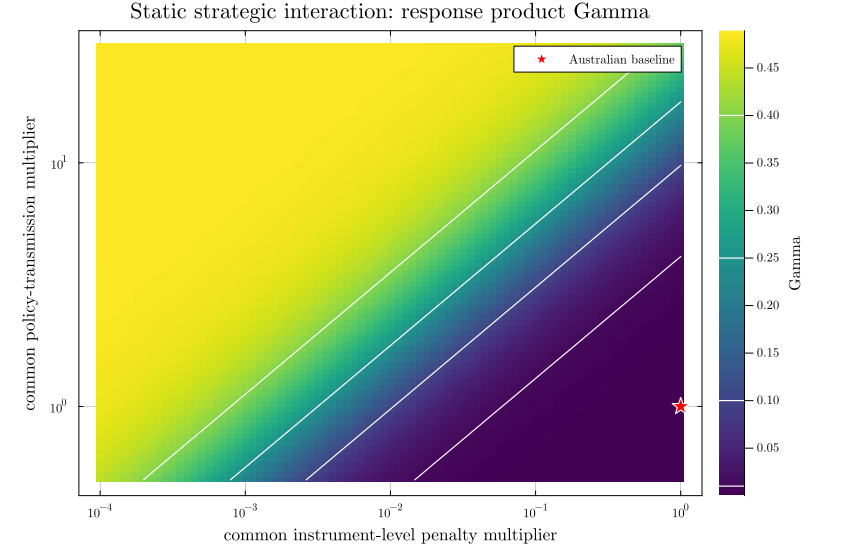
\includegraphics[width=0.83\textwidth]{analytical_interaction_map.png}
\caption{Static response-product ranges before solving the recursive game.}
\label{fig:analyticalstatic}
\end{figure}

\subsection{Dynamic commitment capacity}

Adjustment costs should also be normalised.  Let $D_i$ denote the one-period
own-action curvature before the adjustment term.  Define
\begin{equation}
p_i=\frac{\lambda_i}{D_i+\lambda_i}\in[0,1).            \label{eq:persistence}
\end{equation}
In a one-step problem, $p_i$ is the coefficient with which the inherited
instrument pulls the current choice back toward its previous value.  It is
therefore a dimensionless measure of commitment capacity.  A raw value such as
$\lambda_i=0.05$ is uninterpretable without $D_i$.

The limiting cases clarify why the strategic motive is generally hump-shaped.
When $p_i=0$, the inherited instrument is not payoff relevant and the specific
lagged-policy commitment channel disappears.  When $p_i$ is close to one, the
instrument is nearly frozen: the position is durable, but the authority has
little ability to move it in response to a shock.  Intermediate values give a
player both durability and manoeuvrability.  The location of the peak is not
universal because it depends on discounting, macro persistence, and the rival's
feedback rule.

Discounting enters directly.  The strategic part of today's first-order
condition is proportional to $\beta_i$: a myopic authority cannot invest in a
future position.  Persistent macro and debt states lengthen the interval over
which the rival's response matters.  Conversely, a transitory shock can still
activate strategic investment, but only through the endogenous policy and debt
states that survive it.

An exact local decomposition is available in the solved Markov game.  Let
$K_j$ be the rival's feedback rule and let $\mathcal H^i_{u_j,t+1}$ denote
authority $i$'s total next-period Hamiltonian derivative with respect to the
rival's action, including continuation value.  The rival-response component
of authority $i$'s current first-order condition is
\begin{equation}
\mathcal S_{i,t}=\beta_i(B_i'K_j')\mathcal H^i_{u_j,t+1}.
                                                               \label{eq:wedge}
\end{equation}
The Julia implementation reports the bounded share
\begin{equation}
\Omega_i=\frac{|\mathcal S_i|}
{|\mathcal S_i|+|\mathcal T_i-\mathcal S_i|},           \label{eq:omega}
\end{equation}
where $\mathcal T_i$ is the entire continuation derivative.  Thus
$\Omega_i$ near zero means that continuation behaviour is mostly ordinary
persistence or own smoothing; values above 0.10 indicate a material strategic
component, and values above 0.25 a strong one.  These last two thresholds are
again reporting conventions, not stability conditions.

Figure \ref{fig:analyticaldynamic} solves the full recursive game over
$\Gamma$ and $p_i$.  Each panel gives one authority adjustment costs while the
other remains flexible.  The result makes the two necessary margins visible.
Moderate persistence alone does little at the Australian value of $\Gamma$.
Material strategic shares emerge in parts of the grid once the response
product reaches several hundredths and become more systematic around
$\Gamma=0.1$--$0.4$.  The relationship is non-monotone because stronger
persistence changes both the rival response and the non-strategic continuation
term.  The asymmetry across panels reflects the different mandates and debt
exposures; it is not imposed by different definitions of the objectives.

A large value of $\Omega_i$ is necessary but not sufficient for a large policy
distortion.  The ratio can rise when the non-strategic continuation term is
close to zero, even if the strategic wedge is small in absolute value.  A
quantitatively important leadership result should therefore satisfy three
checks together: material $\Gamma$, material $\Omega_i$, and a visible change
in equilibrium actions or welfare relative to flexible Nash.

\begin{figure}[H]
\centering
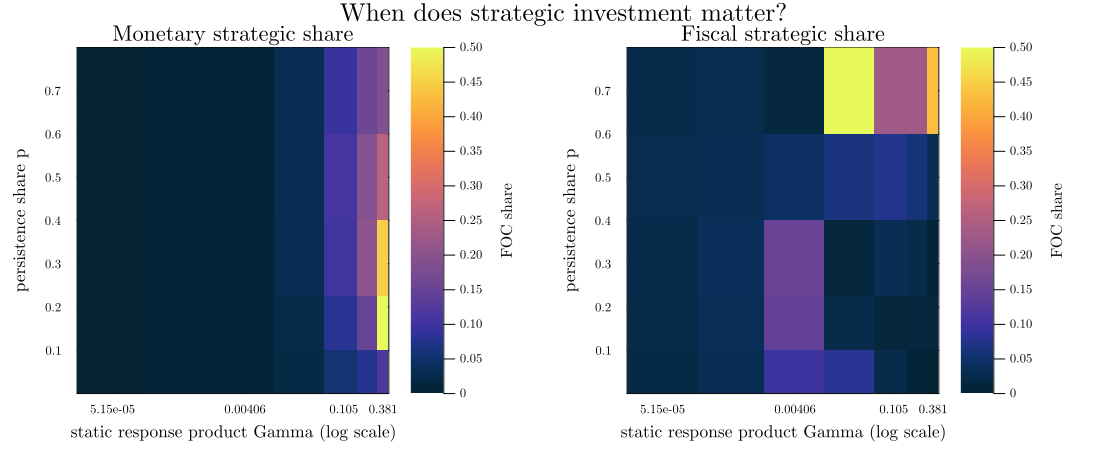
\includegraphics[width=0.95\textwidth]{dynamic_strategic_ranges.png}
\caption{Envelope-based strategic shares over interaction and persistence ranges.}
\label{fig:analyticaldynamic}
\end{figure}

The practical implication is sharp.  To generate a Petkov-style leader effect,
one should not search over $\lambda_i$ in isolation.  First establish that the
static or continuation response product is non-negligible; then vary the
dimensionless persistence share; finally verify that \eqref{eq:wedge}, rather
than the full continuation term, is large.  This sequence prevents ordinary
policy inertia from being mistaken for strategic investment.

\section{Australian calibration}

The quarterly macro coefficients are descriptive OLS estimates for
1993Q1--2019Q4 carried over from the companion Australian data pipeline.  The
source series are the Reserve Bank of Australia's public statistical tables
\citep{RBAData}:
consumer prices (G1), GDP and income (H1), demand and income (H2), and interest
rates (F1.1).  The output gap is constructed from real GDP, the inflation gap
from CPI inflation, the monetary instrument from the real cash-rate gap, and
the fiscal instrument from public-demand deviations.  These are not causal
policy multipliers.  The debt block, loss weights, and adjustment costs are
transparent calibrations.

\begin{table}[H]
\centering
\caption{Baseline quarterly calibration}
\label{tab:calibration}
\begin{tabular}{lll}
\toprule
Parameter & Value & Interpretation\\
\midrule
$\rho_x$ & 0.62875 & output-gap persistence\\
$\rho_\pi$ & 0.56255 & inflation persistence\\
$\sigma$ & 0.03695 & monetary transmission to output\\
$\psi$ & 0.05142 & fiscal transmission to output\\
$\kappa$ & 0.15511 & Phillips-curve slope\\
$\rho_b$ & 0.995 & debt persistence\\
$(\chi_m,\chi_f,\chi_\pi)$ & $(0.015,0.060,0.100)$ & debt transmission\\
$(\lambda_M,\lambda_F)$ & $(0.050,0.040)$ & adjustment-cost primitives\\
$(\omega^M_\pi,\omega^M_x)$ & $(1.50,0.25)$ & monetary mandate\\
$(\omega^F_\pi,\omega^F_x)$ & $(0.50,0.75)$ & fiscal mandate\\
$(\omega^S_\pi,\omega^S_x)$ & $(1.00,0.50)$ & true social objective\\
\bottomrule
\end{tabular}
\end{table}

The impulse experiments use a one-standard-deviation demand contraction of
\DemandSD\ and a cost-push shock of \SupplySD.  Later innovations are zero.
Because the model is linear--quadratic, additive shock variances do not change
the stationary policy gains under certainty equivalence.

The analytical indices immediately locate this calibration.  The static
response product is only $\BaselineGamma$, well inside the negligible range,
whereas the persistence shares are $p_M=\BaselinePersistenceM$ and
$p_F=\BaselinePersistenceF$.  Thus commitment capacity is already moderate;
weak cross-authority interaction is the binding margin.  Holding the
composition of macro transmission fixed, reaching $\Gamma=0.10$ would require
both direct instrument penalties to fall to approximately
\GammaTenPenaltyScale\ of baseline, or both policy-transmission vectors to be
about \GammaTenTransmissionScale\ times their estimated size.  These are large
counterfactual movements, not plausible confidence intervals around the OLS
coefficients.  In the bilateral demand-shock game, the exact bounded strategic
shares are only \BaselineMonetaryWedgeShare\ for monetary policy and
\BaselineFiscalWedgeShare\ for fiscal policy.  This establishes analytically
and numerically why the baseline mainly displays smoothing rather than
endogenous leadership.

\section{Results}

\subsection{Static leadership and dynamic policy positions}

Figure \ref{fig:map} is the most direct diagnostic.  Diamonds show static Nash,
the two Stackelberg orders, and static cooperation.  Circles show shock-period
actions from the recursive regimes.  Monetary persistence mainly reduces the
absolute monetary movement; fiscal persistence mainly reduces the fiscal
movement.  When both costs are present, both adjustments occur.

\begin{figure}[H]
\centering
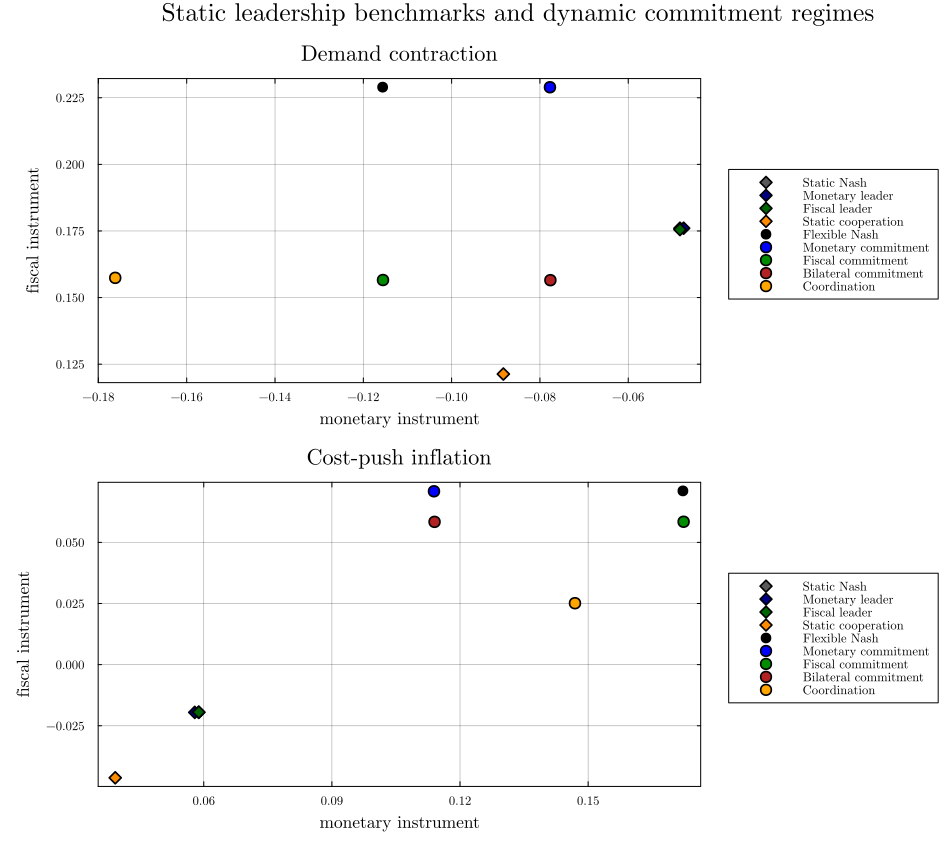
\includegraphics[width=0.82\textwidth]{policy_benchmark_map.png}
\caption{Static policy benchmarks and initial actions from the recursive game.}
\label{fig:map}
\end{figure}

For the demand shock, monetary persistence closes
\DemandMonActionIndex\ of the flexible-Nash action distance to the monetary
leader, while fiscal persistence closes \DemandFisActionIndex\ toward the
fiscal leader.  The corresponding cost-push figures are
\SupplyMonActionIndex\ and \SupplyFisActionIndex.  These movements are
consistent with commitment capacity, but they cannot by themselves identify
which authority has become leader: the monetary-leader and fiscal-leader
points differ by only \DemandLeaderSeparation\ after the demand shock and
\SupplyLeaderSeparation\ after the cost-push shock.  The proximity indices are
diagnostics, not structural estimates of leadership.

Figure \ref{fig:ruleproximity} makes the same warning visible in full
feedback-rule space.  Fiscal adjustment costs produce the larger shift at the
baseline.  Because both leader targets are nearly coincident, movement toward
one is almost automatically movement toward the other.

\begin{figure}[H]
\centering
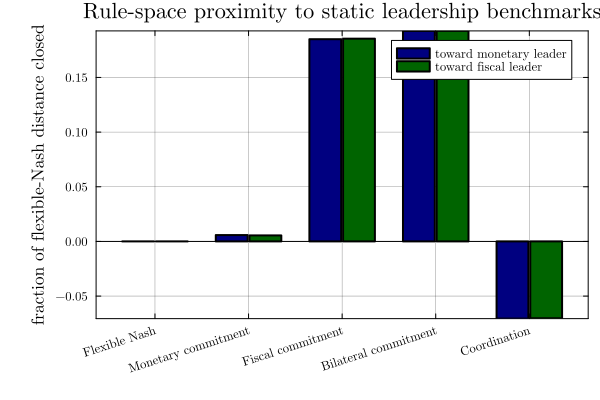
\includegraphics[width=0.82\textwidth]{leadership_indices.png}
\caption{Distance of complete feedback rules from the static benchmarks.}
\label{fig:ruleproximity}
\end{figure}

\subsection{Shock dynamics and the policy mix}

Figures \ref{fig:demand} and \ref{fig:supply} show 16 quarters of the two
impulse responses.  Every policy authority reoptimizes in every quarter.  The
paths are therefore recursive Markov strategies, not commitments to an
open-loop sequence.  Adjustment costs operate through the inherited policy
states in \eqref{eq:state}.

\begin{figure}[H]
\centering
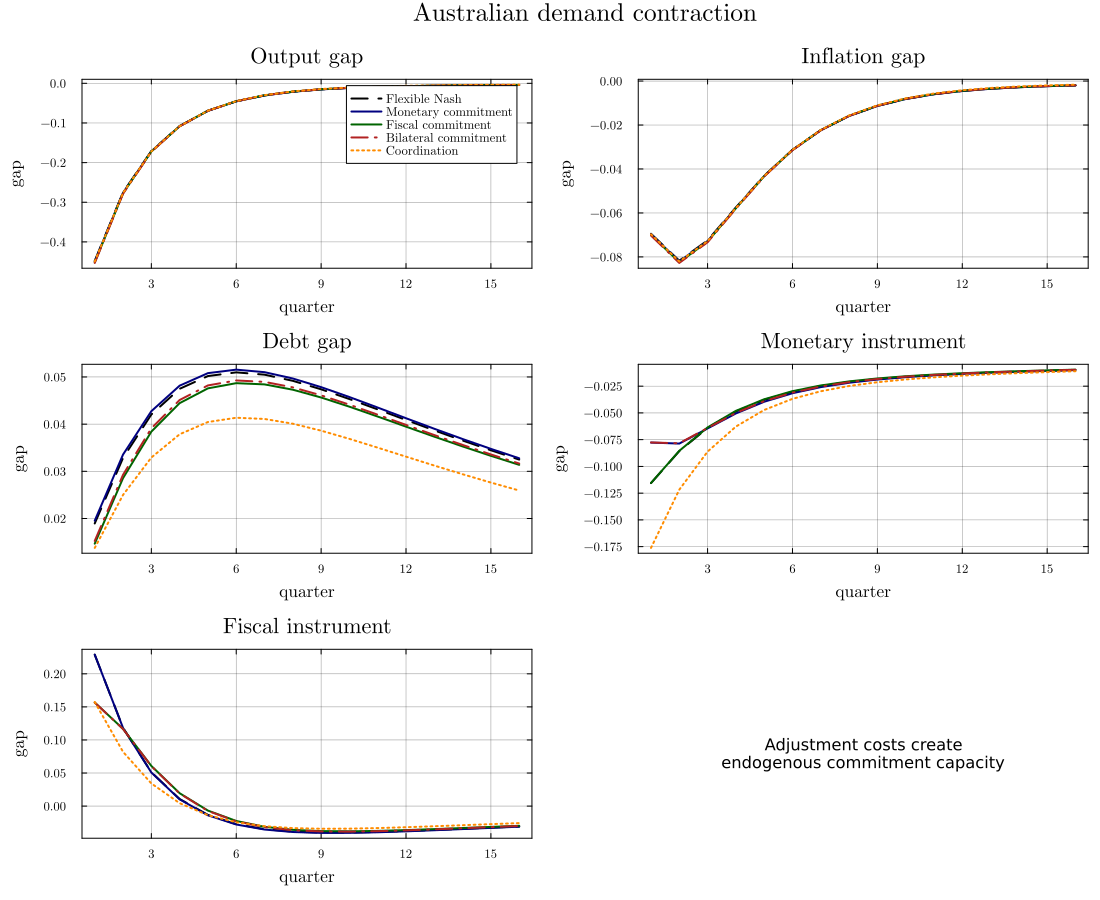
\includegraphics[width=0.95\textwidth]{demand_commitment_paths.png}
\caption{Recursive responses to an Australian demand contraction.}
\label{fig:demand}
\end{figure}

\begin{figure}[H]
\centering
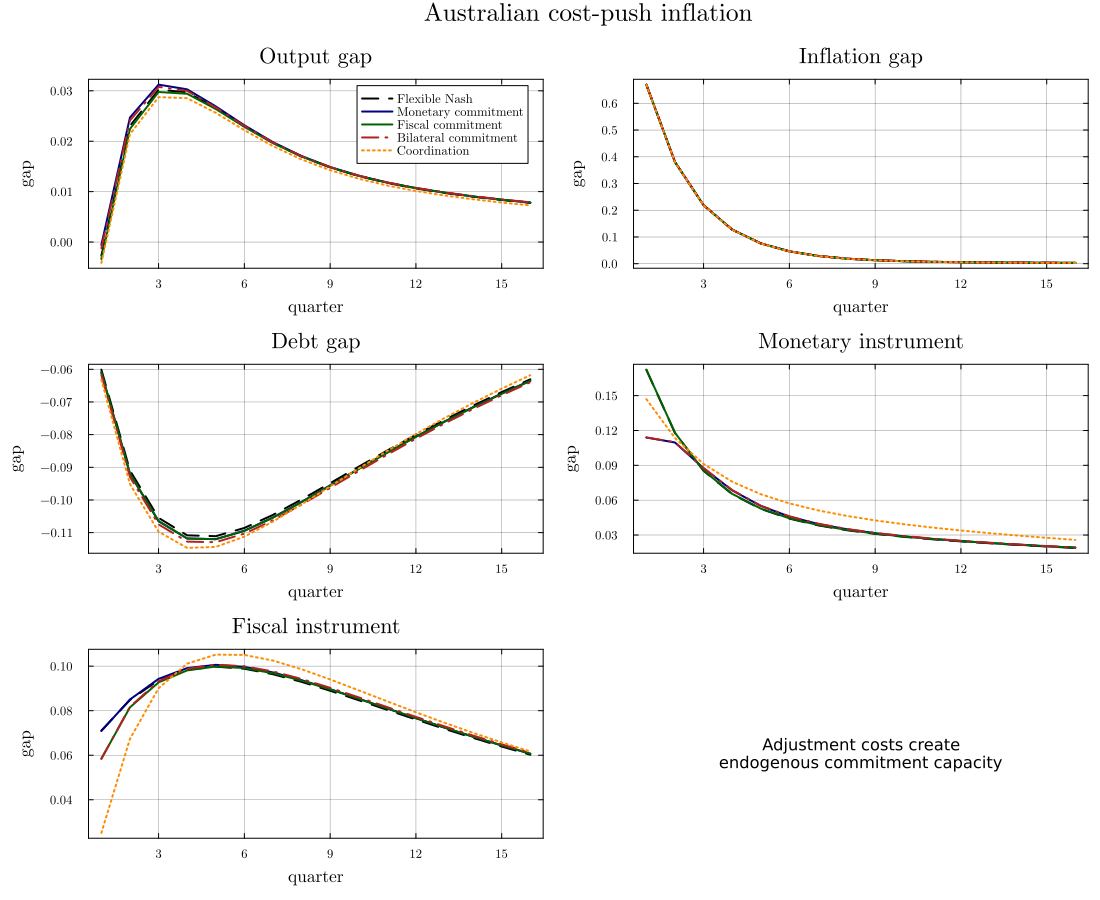
\includegraphics[width=0.95\textwidth]{cost_push_commitment_paths.png}
\caption{Recursive responses to an Australian cost-push shock.}
\label{fig:supply}
\end{figure}

Table \ref{tab:initial} reports the initial policy choices.  The flexible game
responds sharply because there is no cost to reversing the instruments next
quarter.  Monetary persistence changes mostly $m_0$; fiscal persistence
changes mostly $f_0$.  Cooperation changes the mix more substantially,
especially fiscal policy after a demand contraction.  This separates two
ideas that were previously conflated: coordination concerns the objective and
joint internalisation of spillovers; commitment capacity concerns the state
dependence of decentralised play.

\begin{table}[H]
\centering
\caption{Initial recursive policy choices}
\label{tab:initial}
\begin{tabular}{lrrrr}
\toprule
&\multicolumn{2}{c}{Demand contraction}&\multicolumn{2}{c}{Cost-push shock}\\
Regime & $m_0$ & $f_0$ & $m_0$ & $f_0$\\
\midrule
Flexible Nash & \DemandFlexibleM & \DemandFlexibleF & \SupplyFlexibleM & \SupplyFlexibleF\\
Monetary persistence & \DemandMonetaryM & \DemandMonetaryF & \SupplyMonetaryM & \SupplyMonetaryF\\
Fiscal persistence & \DemandFiscalM & \DemandFiscalF & \SupplyFiscalM & \SupplyFiscalF\\
Bilateral persistence & \DemandBothM & \DemandBothF & \SupplyBothM & \SupplyBothF\\
Coordination & \DemandCoordM & \DemandCoordF & \SupplyCoordM & \SupplyCoordF\\
\bottomrule
\end{tabular}
\end{table}

\subsection{Welfare and bilateral commitment capacity}

For comparability, Table \ref{tab:loss} uses a common macro-welfare yardstick:
the true social objective excluding adjustment-resource costs.  Actual social
loss, including those costs, is also written to the output CSV.  The common
loss prevents a regime from looking worse merely because a newly introduced
physical cost is counted in one column but absent in another.

\begin{table}[H]
\centering
\caption{Forty-quarter common macro loss}
\label{tab:loss}
\begin{tabular}{lrr}
\toprule
Regime & Demand contraction & Cost-push shock\\
\midrule
Flexible Nash & \DemandFlexibleLoss & \SupplyFlexibleLoss\\
Monetary persistence & \DemandMonetaryLoss & \SupplyMonetaryLoss\\
Fiscal persistence & \DemandFiscalLoss & \SupplyFiscalLoss\\
Bilateral persistence & \DemandBothLoss & \SupplyBothLoss\\
Coordination & \DemandCoordLoss & \SupplyCoordLoss\\
\bottomrule
\end{tabular}
\end{table}

Monetary persistence slightly raises the common demand-shock loss, while the
baseline fiscal persistence slightly lowers it.  This is not paradoxical.
Smoothing can either impede timely stabilisation or restrain an excessively
aggressive delegated response.  It is also not a general welfare ranking,
because the physical implementation costs have deliberately been omitted from
this comparison.

Figure \ref{fig:sensitivity} varies one adjustment cost at a time.  Fiscal
persistence initially brings the feedback rule closer to the static leader
region and lowers the macro loss, but the relationship is non-monotone.
Monetary persistence ceases to look leader-like at higher costs.  A sufficiently
large adjustment penalty freezes an instrument; it does not grant unlimited
first-mover power.

\begin{figure}[H]
\centering
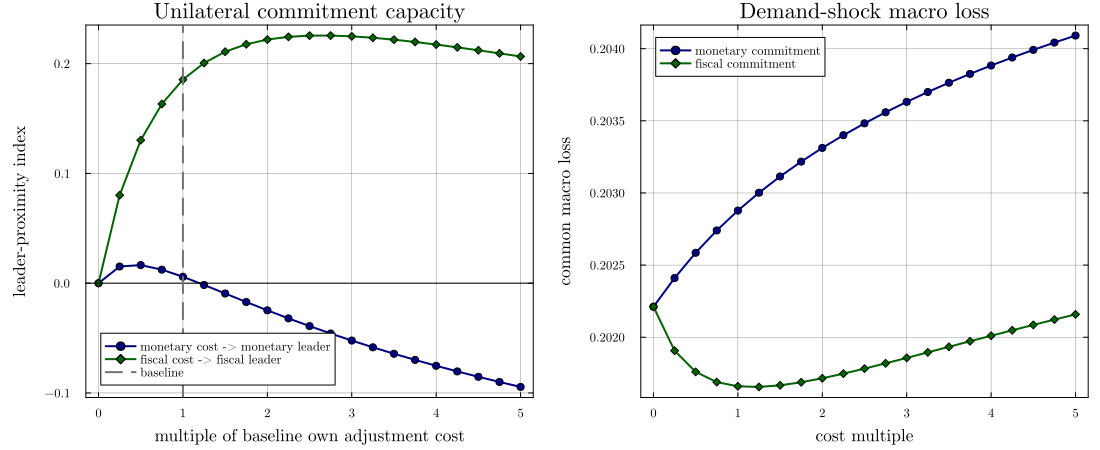
\includegraphics[width=0.95\textwidth]{unilateral_commitment_sensitivity.png}
\caption{Unilateral commitment capacity and demand-shock loss.}
\label{fig:sensitivity}
\end{figure}

When both capacities vary, Figure \ref{fig:metapolicy} shows nearly separable
effects on the two initial actions.  Figure \ref{fig:metawelfare} shows the
associated welfare surface.  The exercise does not reveal the strong mutual
escalation associated with a Stackelberg-warfare point.  That absence is
consistent with the small follower slopes in \eqref{eq:slopes}.

\begin{figure}[H]
\centering
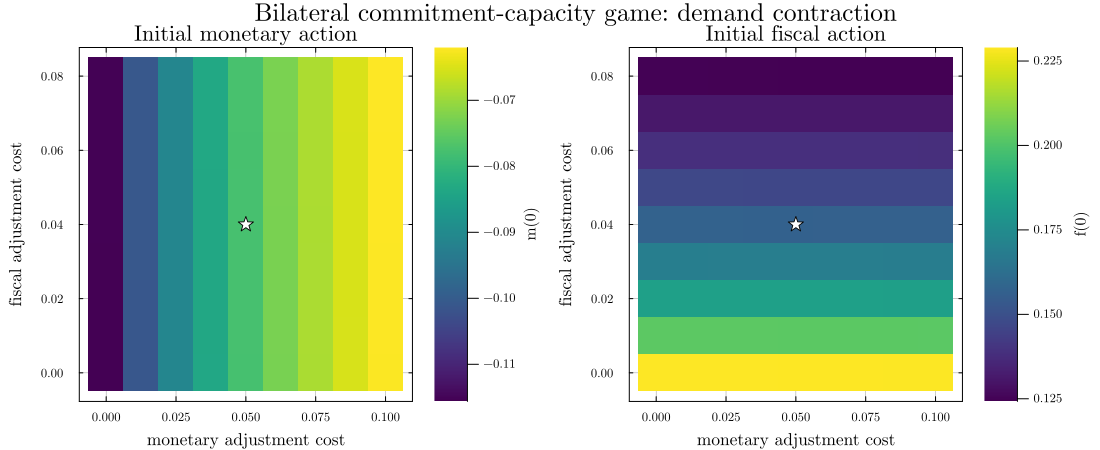
\includegraphics[width=0.95\textwidth]{meta_nash_policy_map.png}
\caption{Initial policy choices as both adjustment-cost primitives vary.}
\label{fig:metapolicy}
\end{figure}

\begin{figure}[H]
\centering
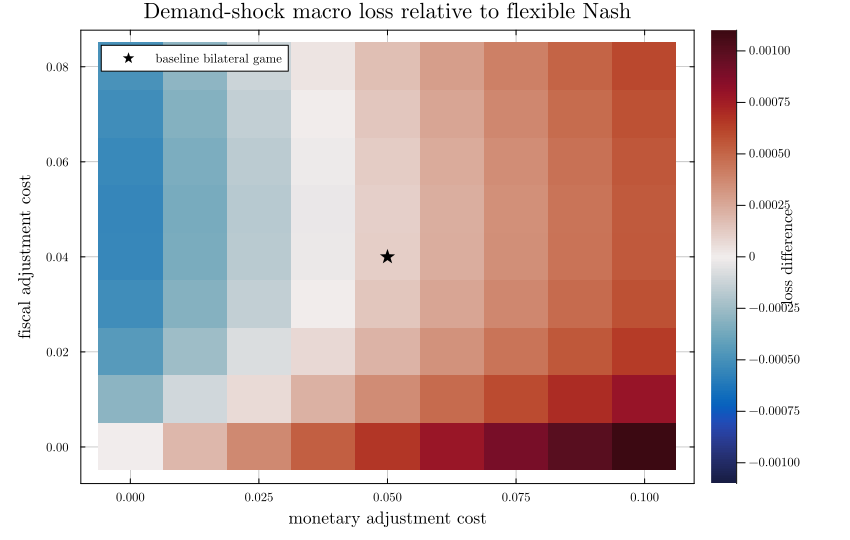
\includegraphics[width=0.82\textwidth]{meta_nash_welfare_map.png}
\caption{Demand-shock macro loss relative to flexible Nash.}
\label{fig:metawelfare}
\end{figure}

\subsection{Stability and equilibrium selection}

The bilateral closed-loop spectral radius is \BilateralRadius, below unity.
All \SearchStarts\ Riccati initialisations converge to the selected rule; the
largest rule distance is \SearchMaxDistance.  Thus the numerical search finds
one stable stationary linear equilibrium at the baseline.  This does not prove
global uniqueness.  Multiple equilibria would require either additional
Riccati roots outside the search basin or nonlinear mechanisms absent from the
local quadratic model.

Strategic complementarity and multiplicity must not be equated.  Positive
best-response slopes can coexist with a unique equilibrium if their product is
small.  In the present calibration the contemporaneous slopes are not only
below the instability threshold but quantitatively close to zero.  The model
therefore shows the importance of coordination without yet generating a hard
equilibrium-selection problem.

\section{Steady state, shocks, and the interpretation of leadership}

With zero gaps, zero shocks, and instruments at their neutral values,
\begin{equation}
s^*=0,\qquad m^*=f^*=0.
\end{equation}
All quadratic marginal losses vanish there.  Adjustment costs also vanish
because neither instrument changes.  There is consequently no realised
strategic-investment wedge at the deterministic steady state, even though the
off-equilibrium feedback derivatives remain part of the policy rules.

A shock activates the mechanism.  The authorities disagree over the desired
mix of output and inflation stabilisation; current controls determine both
macro states and inherited instruments; future policymakers respond to those
states.  Nominal rigidity, represented here by inflation persistence and the
Phillips curve, determines how long the disagreement remains payoff relevant.
The appropriate solution is therefore a Markov-perfect feedback game, not an
open-loop equilibrium.

The current approach captures the strategic-investment mechanism in a narrow,
transparent way.  It does not yet capture commitment through private-sector
expectations.  In a fully forward-looking New Keynesian block,
\begin{align*}
x_t&=E_tx_{t+1}-\sigma(m_t-E_t\pi_{t+1})+\psi f_t+d_t,\\
\pi_t&=\beta E_t\pi_{t+1}+\kappa x_t+u_t,
\end{align*}
future policy rules change current behaviour directly.  That extension could
amplify the strategic channel and change the ranking of commitment devices.

\section{Forward-looking New Keynesian extension}
\label{sec:nk}

\subsection{Private behaviour and the homotopy}

The backward-looking block isolates policy-state investment but omits the
effect of expected future policy on private behaviour today.  The standard New
Keynesian IS curve and Phillips curve make that channel explicit
\citep{ClaridaGaliGertler1999}.  To distinguish forward-looking behaviour from
unrelated recalibration, introduce $\theta\in[0,1]$:
\begin{align}
x_t={}&(1-\theta)\rho_xx_{t-1}+\theta E_tx_{t+1}
-\sigma\{m_t-(1-\theta)\pi_{t-1}-\theta E_t\pi_{t+1}\}
+\psi f_t+d_t,                                           \label{eq:nkis}\\
\pi_t={}&(1-\theta)\rho_\pi\pi_{t-1}
+\theta\beta_pE_t\pi_{t+1}+\kappa x_t+u_t.             \label{eq:nkpc}
\end{align}
At $\theta=0$, equations \eqref{eq:nkis}--\eqref{eq:nkpc} reproduce the
empirical block in \eqref{eq:is}--\eqref{eq:pc}.  At $\theta=1$, they become
the pure forward-looking NK equations.  The debt transition, mandates,
adjustment costs, and shock sizes are unchanged.  Thus $\theta$ is a diagnostic
homotopy, not an estimated structural parameter.

Suppose the private sector conjectures
\begin{equation}
\begin{bmatrix}x_t\\\pi_t\end{bmatrix}=G s_t.           \label{eq:G}
\end{equation}
Given $G$, expected future output and inflation are $Gs_{t+1}$.  Substitution
into \eqref{eq:nkis}--\eqref{eq:nkpc} yields
\begin{equation}
s_{t+1}=A(G)s_t+B_M(G)m_t+B_F(G)f_t.                    \label{eq:nkreduced}
\end{equation}
The authorities solve the simultaneous Markov-perfect game conditional on
$G$.  If their rules are $K_M(G)$ and $K_F(G)$ and the contemporaneous private
response is $O(G)[s_t',m_t,f_t]'$, rational expectations require
\begin{equation}
G=O_s(G)+O_m(G)K_M(G)+O_f(G)K_F(G).                     \label{eq:nkfixed}
\end{equation}
The Julia solver iterates between the coupled Riccati policy problem and
\eqref{eq:nkfixed}, using continuation in $\theta$ and damping of expectations.
The rule-coefficient error at $\theta=0$ relative to the original solver is
\NKBackwardMatch, an exact implementation check.

Monetary and fiscal authorities move simultaneously with one another.
Households and price setters observe current instruments, understand the
stationary future rules, and form rational expectations.  Future policymakers
therefore affect current outcomes through private beliefs, while current
policymakers affect future incentives through debt, macro states, and inherited
instruments.  This is the two-way strategic channel emphasised in work on
discretionary equilibrium multiplicity \citep{KirsanovaYates2025}.

\subsection{Separating three channels}

Forward-looking behaviour requires a refinement of the strategic
decomposition.  The rival-response term in \eqref{eq:wedge} can be written
\begin{equation}
\mathcal S_{i,t}=\beta_i\sum_h B_{i,h}K_{j,h}
\mathcal H^i_{u_j,t+1}.                                \label{eq:nkdecomp}
\end{equation}
The implementation separates three objects:
\begin{enumerate}
  \item the \emph{macro-state channel}, through future $x$, $\pi$, and debt;
  \item the \emph{adjustment-state channel}, through $m_t$ becoming
        $m_{t-1}$ or $f_t$ becoming $f_{t-1}$ next period; and
  \item the \emph{private-expectations channel}, through current $x_t$ and
        $\pi_t$ depending on the expected future policy rule.
\end{enumerate}
Only the second is the narrow Petkov-style strategic investment created by an
instrument-adjustment cost.  The first exists with flexible instruments
because policy changes future macro states.  The third transmits both types of
intertemporal strategy from the future back into the present.  Calling the
complete continuation derivative ``strategic investment'' would therefore
overstate the role of adjustment costs.

\subsection{How forward-looking behaviour changes the game}

Figure \ref{fig:nktheta} traces demand-shock equilibria.  The mapping from
$\theta$ to policy is strongly non-monotone.  As forward-looking behaviour
first rises, monetary easing becomes larger and fiscal expansion initially
increases.  Beyond about $\theta=0.6$, the fiscal response falls sharply and
changes sign.  At the pure NK endpoint, flexible Nash chooses
$(m_0,f_0)=(\NKFlexibleM,\NKFlexibleF)$, while bilateral persistence chooses
$(\NKBilateralM,\NKBilateralF)$.  Fiscal policy contracts after the transitory
demand shock: anticipated monetary easing and future stabilisation substitute
for a current fiscal expansion, while debt and inflation costs remain.

\begin{figure}[H]
\centering
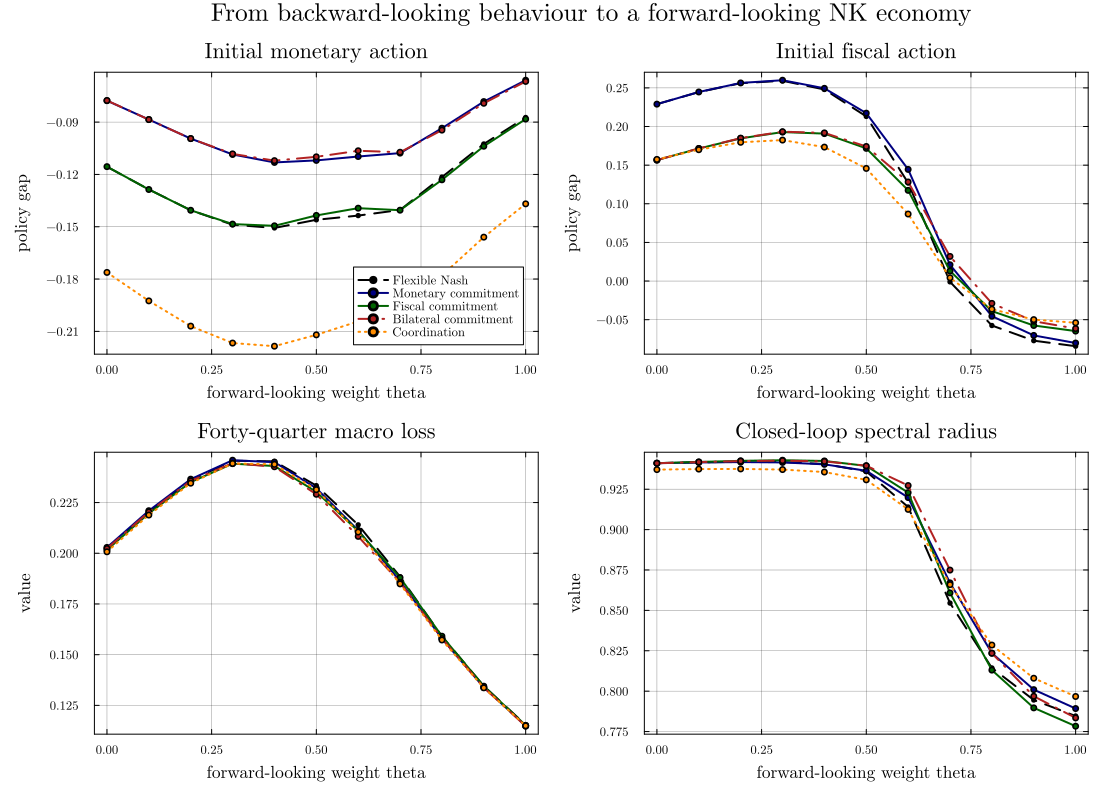
\includegraphics[width=0.96\textwidth]{nk_forwardness_sensitivity.png}
\caption{Policy, welfare, and stability along the forward-looking homotopy.}
\label{fig:nktheta}
\end{figure}

Figure \ref{fig:nkchannels} gives the main strategic-investment result.
Forward-looking behaviour can amplify the adjustment-state wedge, but the
effect is hump-shaped.  The monetary wedge peaks around
$\theta=\NKMonPeakTheta$ at \NKMonPeakWedge; the fiscal wedge peaks around
$\theta=\NKFisPeakTheta$ at \NKFisPeakWedge.  At $\theta=1$, the bounded
adjustment-state shares have fallen to \NKMonInvestmentShare\ and
\NKFisInvestmentShare.  Private expectations therefore do not mechanically
turn instrument smoothing into Stackelberg leadership.  They strengthen the
channel most when policy positions remain persistent enough to matter but
private responses have not already absorbed the future adjustment.

\begin{figure}[H]
\centering
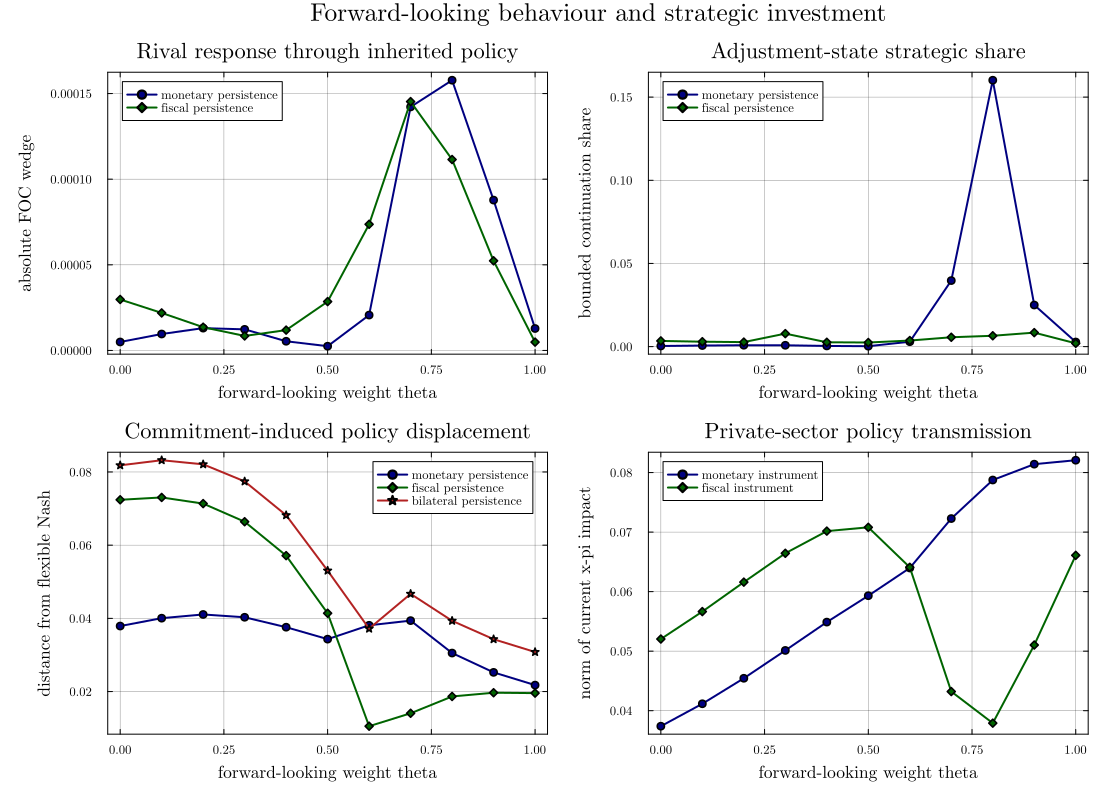
\includegraphics[width=0.96\textwidth]{nk_strategic_investment_channels.png}
\caption{Adjustment-state, macro-state, and private-expectations channels.}
\label{fig:nkchannels}
\end{figure}

The commitment-induced policy displacement becomes smaller at the pure NK
endpoint.  This is consistent with the general finding that the sign and
strength of monetary--fiscal interaction depend on shocks, structural
transmission, and policy inertia rather than mandate differences alone
\citep{MuscatelliEtAl2004}.  Expectations reverse the fiscal sign after a
demand disturbance but do not produce an analogous common reversal after a
cost-push shock.

The pure-NK impulse responses are shown in Figures \ref{fig:nkdemand} and
\ref{fig:nksupply}.  The demand innovation is transitory, so output and
inflation move mostly on impact; debt and inherited policies carry its effects
forward.  The cost-push shock creates more persistent output and debt responses
through anticipated stabilisation policy.

\begin{figure}[H]
\centering
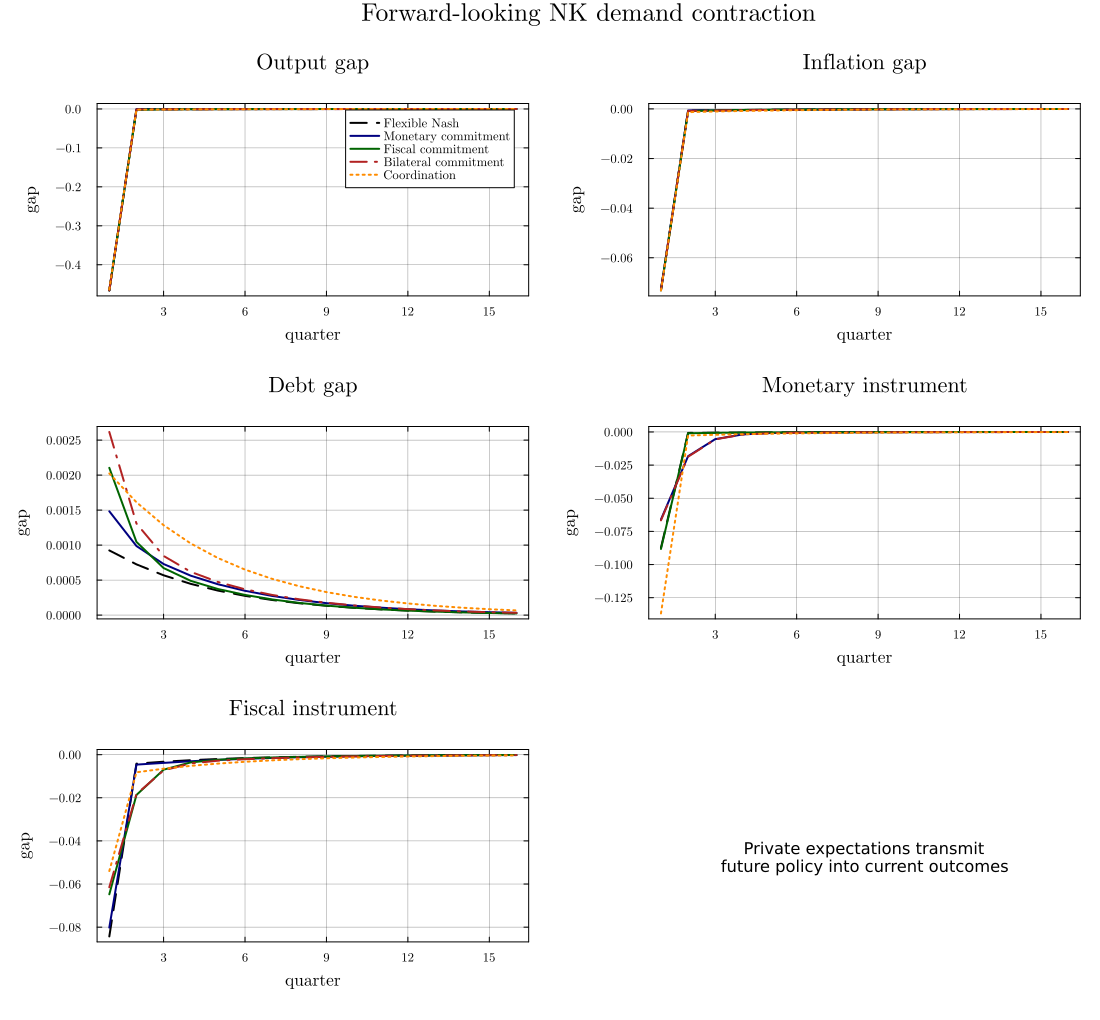
\includegraphics[width=0.95\textwidth]{nk_demand_irfs.png}
\caption{Pure forward-looking NK responses to a demand contraction.}
\label{fig:nkdemand}
\end{figure}

\begin{figure}[H]
\centering
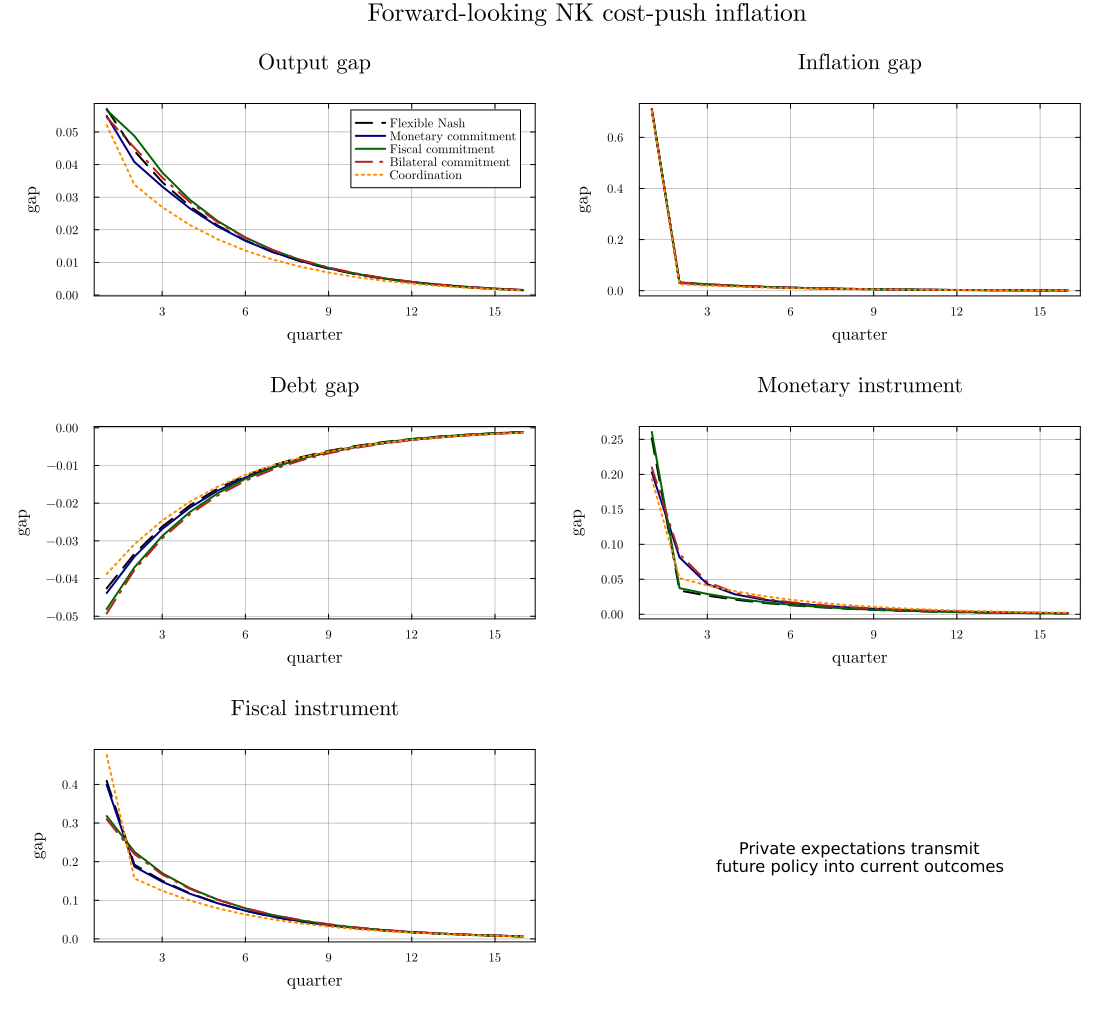
\includegraphics[width=0.95\textwidth]{nk_cost_push_irfs.png}
\caption{Pure forward-looking NK responses to a cost-push shock.}
\label{fig:nksupply}
\end{figure}

For the pure-NK demand experiment, common macro loss is \NKFlexibleLoss\ under
flexible Nash, \NKBilateralLoss\ under bilateral persistence, and
\NKCoordLoss\ under discretionary coordination.  The bilateral regime has a
slightly lower macro-only loss than the flexible social planner because policy
inertia supplies partial commitment.  Once physical adjustment costs are
included, coordination again has the lowest actual social loss.  An institution
can improve stabilisation by constraining future discretion while still
consuming implementation resources.

\subsection{Multiplicity and interpretation}

Forward-looking behaviour makes equilibrium selection a genuine concern.
Different beliefs about future rules can validate different current private
responses and policy choices.  \citet{KirsanovaYates2025}, for example, obtain
multiple stable discretionary equilibria in an NK model with capital, where
private expectations transmit strategic complementarity between current and
future policymakers.

That result is possible, not automatic.  Here \NKSearchAttempts\ dispersed
initial expectations converge to \NKDistinctSolutions\ stable pure-NK
bilateral equilibrium.  Closed-loop roots remain inside the unit circle along
the homotopy.  Expectations materially change the policy mix and create an
intermediate strategic-amplification region without generating numerical
evidence of multiplicity.  The weak response product identified in Section
\ref{sec:ranges} remains a binding limitation.

This is not a global uniqueness theorem.  The search covers linear stationary
equilibria reachable by the damped fixed-point algorithm.  Stronger debt
valuation, persistent shocks, lower instrument penalties, capital
accumulation, or nonlinear fiscal limits could create additional branches.
Those are now well-defined extensions rather than being confounded with the
adjustment-cost mechanism itself.

\section{Relation to monetary--fiscal and fiscal-dominance literatures}

Dynamic monetary--fiscal games distinguish cooperation, discretionary
feedback, and commitment \citep{OudizSachs1984,Tabellini1986}.  Public debt is
especially important because fiscal choices can change a persistent state to
which monetary policy later responds \citep{BeetsmaBovenberg1997}.  The present
debt equation contains that strategic-state channel.

The model does not, however, fully nest the fiscal theory of the price level or
strong fiscal dominance.  That requires nominal government liabilities, a
consolidated intertemporal government budget constraint, and explicit monetary
and fiscal backing regimes.  Here inflation reduces the debt gap and both
authorities respond to debt, so fiscal pressure can influence monetary policy;
but the price level is not selected to satisfy a nominal valuation equation.
The model should therefore be described as a dynamic policy-coordination game
with a fiscal-pressure channel, not as a complete fiscal-dominance model.

The distinction between delegated objectives and social welfare is also
standard in monetary economics.  Rogoff-style conservatism deliberately gives
the central bank a different inflation weight from society, while the social
objective remains fixed.  In the present application, the fiscal authority is
relatively output-oriented and monetary policy relatively inflation-oriented.
Those different weights create conflict, but conflict alone need not create a
large leader advantage.  Transmission and reaction slopes determine whether
one authority can use persistence to manipulate the other.

\section{Conclusion}

The requested dynamic game is a recursive, simultaneous policy game with
lagged instruments as endogenous states.  It differs from the original static
Stackelberg game, while retaining the latter as a benchmark.  With only one
adjustment cost, that authority possesses unilateral commitment capacity; with
both, both authorities try to shape the state inherited by future policymakers.
The model therefore implements the strategic-investment logic discussed by
Petkov and by Jun and Vives.

The Australian baseline does not generate a strong endogenous leader.  The
reason is economic rather than computational: the static follower responses
are weak, and the two leader allocations are nearly coincident.  Adjustment
costs mainly generate own-instrument inertia.  Cooperation still matters for
the policy mix, but the stationary linear game has one numerically detected
stable equilibrium rather than an equilibrium-selection problem.

Forward-looking private behaviour changes the policy mix substantially and
temporarily amplifies the adjustment-state wedge at intermediate values of the
homotopy.  It does not monotonically magnify strategic investment, and the pure
NK endpoint again has small adjustment-specific shares and one detected stable
equilibrium.  Expectations are a conduit, not an independent guarantee of
leadership or multiplicity.

The next useful experiment is therefore not to raise adjustment costs
indiscriminately.  It is to strengthen and estimate the economically relevant
cross-effects: policy transmission, debt valuation, shock persistence, and
mandate divergence.  Adding capital or nominal government liabilities would
then test whether a stronger endogenous state creates additional
rational-expectations equilibrium branches.

\appendix
\section{Reproduction}

All model calculations and figures are generated in Julia.  From this folder:
\begin{verbatim}
julia --project=. -e "using Pkg; Pkg.instantiate(; update_registry=false)"
julia --project=. run_model.jl
julia --project=. run_nk_extension.jl
julia --project=. runtests.jl
julia --project=. runtests_nk.jl
julia --project=. build_tex.jl
\end{verbatim}
The first model command writes calibration, policy rules, equilibrium-search
diagnostics, summary tables, and figures to \texttt{output/}.  The final
command uses the artifact-pinned Tectonic binary to compile this source into
\texttt{STRATEGIC\_INVESTMENT\_POLICY\_GAME.pdf}.

\section{What the numerical checks establish}

The test suite verifies the static Nash first-order conditions, each
Stackelberg follower condition, ownership of the adjustment costs, convergence
and stability of every stationary regime, irrelevance of inherited instrument
states when adjustment costs are zero, activation of those states when costs
are positive, multi-start agreement, and finite simulated losses.  These tests
establish internal numerical consistency.  They do not establish structural
identification of the calibrated weights or global equilibrium uniqueness.
The NK suite additionally verifies the exact $\theta=0$ replication, both
forward-looking private equations at an arbitrary state, the rational-
expectations fixed point, the channel decomposition, and convergence from
dispersed initial beliefs.

\begin{thebibliography}{99}

\bibitem[Beetsma and Bovenberg(1997)]{BeetsmaBovenberg1997}
Beetsma, R. M. W. J. and A. L. Bovenberg (1997).
Central bank independence and public debt policy.
\emph{Journal of Economic Dynamics and Control} 21, 873--894.
\url{https://doi.org/10.1016/S0165-1889(97)00003-1}.

\bibitem[Clarida, Gal\'i and Gertler(1999)]{ClaridaGaliGertler1999}
Clarida, R., J. Gal\'i and M. Gertler (1999).
The science of monetary policy: a New Keynesian perspective.
\emph{Journal of Economic Literature} 37, 1661--1707.
\url{https://doi.org/10.1257/jel.37.4.1661}.

\bibitem[Coury and Petkov(2010)]{CouryPetkov2010}
Coury, T. and V. Petkov (2010).
Monetary delegation: credibility through dynamic incentives.
Dubai Initiative Working Paper, Harvard Kennedy School.
\url{https://www.belfercenter.org/publication/monetary-delegation-credibility-through-dynamic-incentives}.

\bibitem[Jun and Vives(2004)]{JunVives2004}
Jun, B. and X. Vives (2004).
Strategic incentives in dynamic duopoly.
\emph{Journal of Economic Theory} 116, 249--281.
\url{https://doi.org/10.1016/j.jet.2003.08.005}.

\bibitem[Kirsanova and Yates(2025)]{KirsanovaYates2025}
Kirsanova, T. and A. Yates (2025).
Multiple equilibria in the absence of commitment.
\emph{Oxford Review of Economic Policy} 41, 404--425.
\url{https://doi.org/10.1093/oxrep/graf022}.

\bibitem[Muscatelli, Tirelli and Trecroci(2004)]{MuscatelliEtAl2004}
Muscatelli, V. A., P. Tirelli and C. Trecroci (2004).
Fiscal and monetary policy interactions: empirical evidence and optimal policy
using a structural New-Keynesian model.
\emph{Journal of Macroeconomics} 26, 257--280.
\url{https://doi.org/10.1016/j.jmacro.2003.11.014}.

\bibitem[Oudiz and Sachs(1984)]{OudizSachs1984}
Oudiz, G. and J. D. Sachs (1984).
International policy coordination in dynamic macroeconomic models.
NBER Working Paper 1417.
\url{https://doi.org/10.3386/w1417}.

\bibitem[Petkov(2004)]{Petkov2004}
Petkov, V. (2004).
Delegated management in dynamic oligopolies.
Econometric Society 2004 Australasian Meetings, paper 79.
\url{https://ideas.repec.org/p/ecm/ausm04/79.html}.

\bibitem[Reserve Bank of Australia(2026)]{RBAData}
Reserve Bank of Australia (2026).
Statistical tables.
\url{https://www.rba.gov.au/statistics/tables/}.

\bibitem[Tabellini(1986)]{Tabellini1986}
Tabellini, G. (1986).
Money, debt and deficits in a dynamic game.
\emph{Journal of Economic Dynamics and Control} 10, 427--442.
\url{https://doi.org/10.1016/S0165-1889(86)80001-X}.

\end{thebibliography}

\end{document}
